%!TEX root = Zusammenfassung.tex

\section{Methoden zur Abhängigkeitsanalyse}
% ---------------------------------------------------------------------------------------------------------------------
\subsection{Konventionelle Abhängigkeitsanalyse} %2017-05-02
\label{sec:konventionelle_abhaengigkeitsanalyse}

\subsubsection{Prinzipielles Vorgehen am Beispiel (\Cref{fig:datenflussgleichungen,fig:beispielprogramm,fig:resultat})}
\label{ssub:prinzipielles_vorgehen_am_beispiel}

\begin{description}
\item[Basisfall] Synthetisierte Attribute für Zuweisungen im Parsebaum
\item[gen$\lbrack S \rbrack$] die Definitionen eines Statements $S$
\item[kill$\lbrack S \rbrack$] solche Definitionen, die von Statement $S$ überschrieben werden.
\item[zusammengesetzte Anweisungen] Verallgemeinerung von $gen[S]$ und $kill[S]$ auf zusammengesetzte Anweisungen wie Sequenz, Konditional und Schleife.
  Dafür ist eine Abschätzung notwendig:
  \begin{description}
    \item[$gen$] es \emph{könnte} generiert worden sein.
    \item[$kill$] es ist \emph{garantiert} gelöscht worden.
  \end{description}
\end{description}

Die Berechnung erfolgt entlang des Parsebaums (bottom-up) durch \emph{Datenflussgleichungen} -- oder allgemein durch Fixpunktiteration.

\begin{figure}[p]
  \centering
  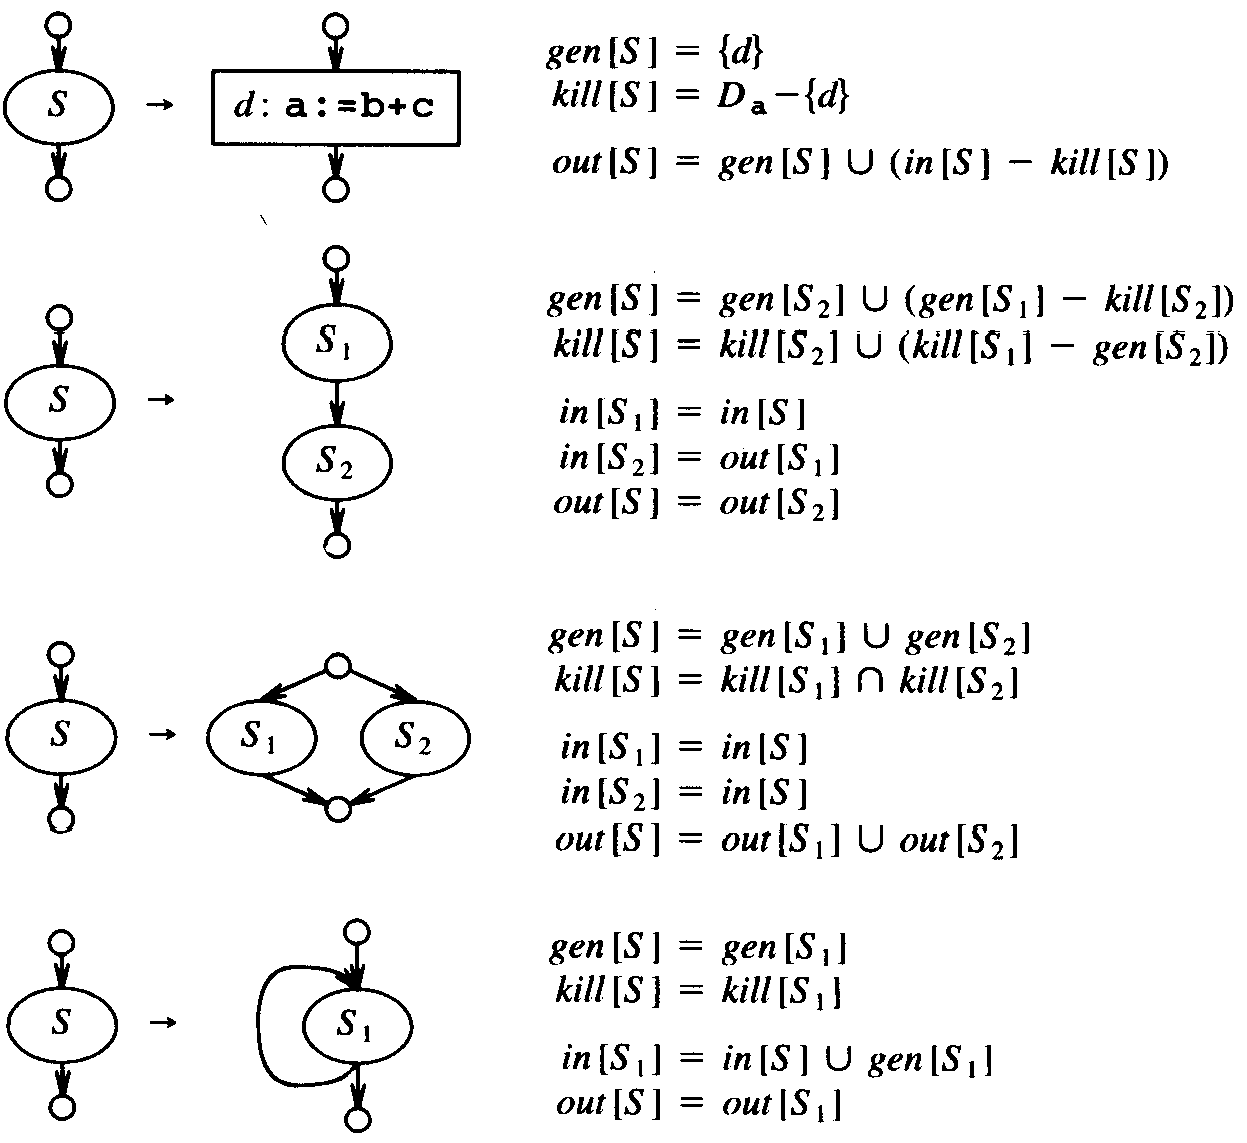
\includegraphics[scale=0.2]{images/bild1-3.png}
  % \caption{Datenflussgleichungen für \glqq erreichende Definitionen\grqq\ }
  \caption{Datenflussgleichungen für zusammengesetzte Anweisungen}
  \label{fig:datenflussgleichungen}
\end{figure}

\begin{figure}[p]
  \centering
  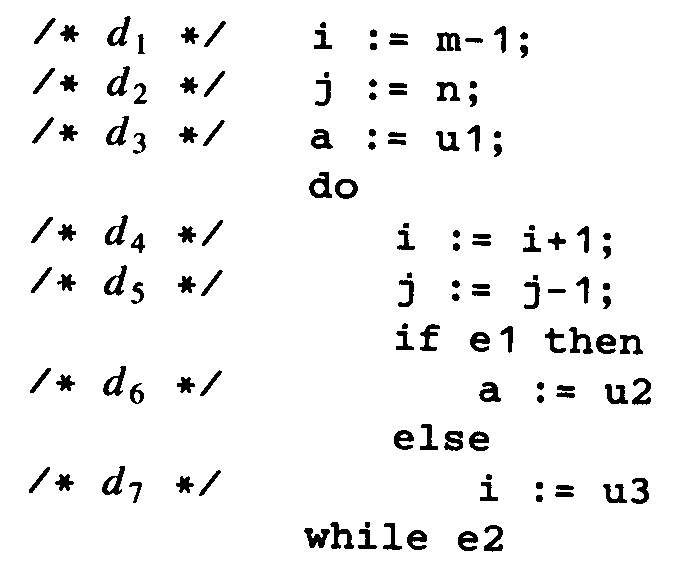
\includegraphics[scale=0.2]{images/bild3-1.png}
  \caption{Beispielprogramm}
  \label{fig:beispielprogramm}
\end{figure}

\begin{figure}[p]
  \centering
  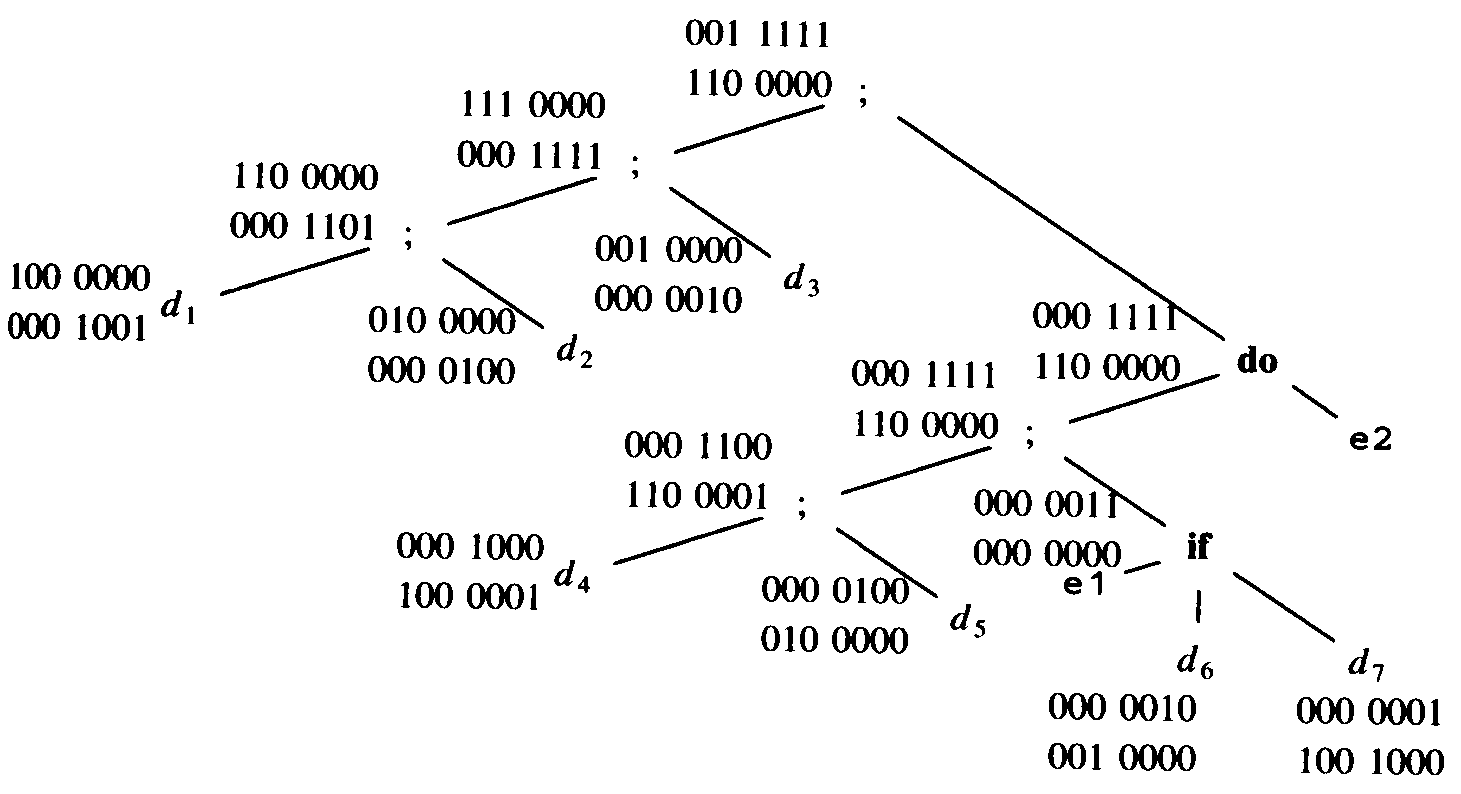
\includegraphics[scale=0.2]{images/bild2-1.png}
  \caption{Resultat der konventionellen Abhängigkeitsanalyse}
  \label{fig:resultat}
\end{figure}

\subsubsection{Nachteile dieses Verfahrens}
\label{ssub:nachteile_dieses_verfahrens}

\begin{itemize}
  \item Bitvektor-Darstellung ungeeignet für Arrays (benötigt ein bit pro Arrayzelle)
  \item teure Mengenoperationen bei sehr großen Bitvektoren
  \item Konflikte, z.\,B. für kill, nur ungenau:
    \begin{itemize}
    \item auf Variablennamen basiert (für Array ungeeignet)
    \item keine Berücksichtigung von eventuell bekannten Schleifengrenzen
    \item keine Berücksichtigung der sequentiellen Ausführungsordnung
    \end{itemize}
  \item für jedes Analyseziel ein neues Datenflussgleichungssystem von Grund auf neu berechnen
  \item im allgemeinen Fall Fixpunktiteration nötig
\end{itemize}

% ---------------------------------------------------------------------------------------------------------------------
\subsection{Polyedermodell}

\subsubsection{Das ursprüngliche Modell}
\label{sec:orig-mod}

\begin{enumerate}
\item Restriktionen:
\begin{enumerate}
\item perfekt verschachtelt
\item Schleifengrenzen: affine Ausdrücke in Strukturparametern und umgebenden
  Indizes und Maxima bzw. Minima davon (für Unter- bzw. Obergrenzen)
\item Arrayindizes affin in den Schleifenindizes und Strukturparametern
\item uniforme Abhängigkeiten
\item ein Schedule und eine Allokation für den kompletten Rumpf;
  Schedule zunächst eindimensional
%\item Schedule und Allokation linear, voneinander lin. unabhängig,
%  gemeinsam volle Dinensionalität
\end{enumerate}
%
\item Modell:
\begin{enumerate}
\item $n$-dimensionaler Schleifensatz im $n$-dimensionalen Raum (je
  Schleife eine Dimension)
\item jeder affine Ausdruck in den Schleifengrenzen definiert einen
  Halbraum
\item Polyeder: der Durchschnitt endlich vieler Halbräume
\item Polytop: beschränktes Polyeder
\item (Quell-)Indexraum ist ein Polytop
\item Abhängigkeiten durch Pfeile im Indexraum repräsentiert
\item Quellpolytop beinhaltet alle nötigen Informationen
\end{enumerate}
%
\item Raum-Zeit-Abbildung:
\begin{enumerate}
\item Schedule: Funktion, die jeder Operation einen (logischen)
  Ausführungszeitpunkt zuordnet, und dabei die durch die Abhängigkeiten
  vorgegebenen Bedingungen berücksichtigt
\item für das Modell: affine Funktion
\item graphische Bestimmung s. Beispiel der Vorlesung
\item mathematische Bestimmung: lineare Programmierung. Aufgabe:
  minimiere die affine Funktion unter der Nebenbedingung, daß ihr Wert
  für einen abhängigen Punkt größer ist als ihr Wert an dem Punkt, von
  dem er abhängt.
\item Allokation: Funktion, die jeder Operation einen (virtuellen)
  Prozessor zur Ausführung zuordnet
\item für das Modell: affine Funktion, die zum Schedule linear
  unabhängig ist (wegen der realen Maschinen und wegen des Modells
  nötig!)
\item Raum-Zeit-Abbildung: die (mehrdimensionale) affine Abbildung,
  repräsentiert durch die Transformationsmatrix, die sich aus Schedule
  und Allokation zusammensetzt, und so jeder Operation einen
  Raum-Zeit-Punkt der Ausführung zuweist. Zusätzliche Restriktion an die
  Allokation: die Raum-Zeit-Matrix muß unimodular sein (Determinante
  betragsmäßig 1)
\end{enumerate}
%
\item Transformation des Modells:
\begin{enumerate}
\item Problem: jede einzelne Dimension kann teilweise in Raum und
  teilweise in der Zeit sein
\item Ziel: Separation -- jede Dimension entweder im Raum oder in der Zeit
\item Weg: Basiswechsel = Anwendung der Raum-Zeit-Abbildung auf den
  Quell-Indexraum
\item Resultat: ``verzerrtes'' Polytop: Zielpolytop
\end{enumerate}
%
\item Zurück zum Programm:
\begin{enumerate}
\item Aufgabe: ``scanning'' der Punkte des Zielpolytops
\item parallele Schleifen für die Raumdimensionen und sequentielle
  Schleifen für die Zeitdimensionen
\item Weg: im Quell-Ungleichungssystem die Indizes durch
  ``$T^{-1}*$Zielindizes'' ersetzen und auflösen
\item abhängig von der gewünschten Reihenfolge der Zieldimensionen:
  (a)synchrones Programm
\item Quellindizes durch ``$T^{-1}*$Zielindizes'' ersetzen
\end{enumerate}
\end{enumerate}

\subsubsection{Das erweiterte Modell}
\label{sec:new-mod}

Erweiterungen:
\begin{enumerate}
\item affine Abhängigkeiten\\[-7mm]
\item stückweise affine Schedules\\[-7mm]
\item per-Statement-Schedule\\[-7mm]
\item nicht-perfekte Verschachtelung\\[-7mm]
\item nicht-unimodulare Raum-Zeit-Abbildungen\\[-7mm]
\item beliebige (z.B. nicht-invertierbare) Raum-Zeit-Abbildungen\\[-7mm]
\item beliebige Schleifentypen\\[-7mm]
\item allgemeine Array-Indizes\\[-7mm]
\end{enumerate}


\subsubsection{Banerjee}

\paragraph{Normalisierung des Schleifenkopfes}

Die Behandlung von Schrittweiten ungleich von eins, insbesondere von
negativen Schrittweiten, macht die Abhängigkeitsanalyse aufwendig. Daher
normalisiert man Schleifen oft wie folgt:



  % {\sf for $i:=x$ to $y$ step $s$ do $R(i)$}

\begin{minipage}{.4\textwidth}
  \begin{algorithm}[H]
      \SetKw{KwStep}{step}
      \For{$i:=x$ \KwTo $y$ \KwStep s}{
        \( R(i) \)
      }
  \end{algorithm}
\end{minipage}
\begin{minipage}{.5\textwidth}
    \qquad $\to$ \qquad
    \begin{algorithm}[H]
          \SetKw{KwStep}{step}
          \For{\( i' := 0\) \KwTo \( \frac{y\!-\!x}{s} \) \KwStep 1}{
            \( R(i' \cdot s + x) \)
          }
      \end{algorithm}
\end{minipage}
  % {\sf for $i':=0$ to ${y\!-\!x}\over s$ step $1$ do $R(i'*s+x)$}
  ~\\
(vgl. \cite{Zima90}, S. 175)

\paragraph{Konflikt-Gleichungssystem}

Zwei Operations $o_s$ und $o_t$ müssen auf dieselbe Speicherzelle
zugreifen, d.h., die Variablennamen und die Array-Indizes, die $o_s$ und
$o_t$ ansprechen, müssen in allen Komponenten übereinstimmen. Für die
entsprechenden Iterationsvektoren $i_s$ und $i_t$ muß also in
Matrixnotation gelten:
$$i_s * A + a_0 = i_t * B + b_0,$$ wobei jede Spalte von $A$ ($B$) die
Koeffizienten eines Array-indexes beinhaltet und $a_0$ ($b_0$) den
konstanten Anteil bechreibt \cite{Ban93}.

Anders notiert: $$(i_s, i_t) * \left( {A \atop -B} \right) = b_0-a_0$$

Lösung wie im Abschnitt für mathematische Grundlagen
beschrieben.

\paragraph{Existenz-Ungleichungssystem}

Die zwei Operations $o_s$ und $o_t$ müssen beide durch das Programm
wirklich generiert werden, d.h., die Iterationsvektoren $i_s$ und $i_t$
müssen im jeweiligen Indexraum der entsprechenden Statements
sein. Matrixnotation: $$p_0 \leq i * P \hbox{\qquad bzw. \qquad} i*Q \leq
q_0$$ für die unteren bzw. oberen Grenzen der Indexräume. Diese
Ungleichungen müssen natürlich sowohl für $i_s$ als auch für $i_t$
aufgestellt werden.

Die -- ggfs. parametrisierten -- Lösungen des Konflikt-Gleichungssystems
kann man in das Ungleichungssystem einsetzen und so die Lösbarkeit
innerhalb des Indexraums überprüfen, bzw. ggfs. die Wahl der Parameter
einschränken.

\paragraph{Ordnungsrelation und Abhängigkeitstypen}

Bis hierher haben wir zwei Operations $o_1$ und $o_2$, die eine
Abhängigkeit verursachen. Frage: Wer ist Quelle, wer Ziel?  Wir wissen:
Operation $o_s$ muß gem.  der sequentiellen Ausführungsreihenfolge vor
$o_t$ ausgeführt werden. Lösung: teile die (ggfs. parametrisierten)
Paare von Iterationsvektoren so in zwei Mengen ein, daß in einer stets
gilt $o_1 \prec o_2$ und in der anderen $o_2 \prec o_1$ (ggfs. unter
Aufteilung der Räume für die Wahl der Parameter). Dadurch sind jeweils
Quelle und Ziel identifiziert, was damit auch die Typen der
Abhängigkeiten lt. Tabelle im vorigen Abschnitt festlegt. (Die Ordnung ist bei dem Verfahren nach Banerjee nicht a priori bekannt.)

\paragraph{Optimierung}
Die Optimierung wird bei Banerjee komplett vernachlässigt.

\paragraph{Randbemerkung: Sonderfälle}
Banerjee stellt Sonderfälle vor, in denen sich die Analyse etwas vereinfacht.
\begin{enumerate}
\item ``regulärer'' Schleifensatz: perfekt, $P=Q$ und $A=B$, dann für $d
  = i_s-i_t$. Dadurch $$ d * A = a_0-b_0 \hbox{\qquad und \qquad} p_0-q_0 \leq
  d*P \leq q_0-p_0$$. Die Halbierung der Variablenzahl macht das
  Gleichungssystem einfacher und die Ordnung handlicher.
\item ``rechteckiger'' Schleifensatz: $P=Q=I_m$ (Identität) und $A$ und
  $B$ in Diagonalform (aber nicht unbeding identisch). Dadurch
  unabhängige $m$ Gleichungen mit je 2 Variablen, die unabhängig
  voneinander aufgelöst werden können. Die Zeilenstufenreduktion wird
  daher etwas übersichtlicher, aber im Endeffekt keine spürbare
  Erleichterung.
\end{enumerate}

% sd
\paragraph{Beispiel zur Abhängigkeitsanalyse nach Banerjee}
\textit{Programmcode:}\\

\begin{procedure}
\SetAlgoLined
\For{$i=10$ \KwTo $200$}{
    \For{$j=7$ \KwTo $167$}{

        \textbf{S:} $X[2i+3, 5j-1, j]$ :=...\\
        \textbf{T:} ... := ... $X[i-1,2i-6,3j+2]$
    }
}
\end{procedure}
~\\
\textit{Konfliktgleichungssystem:} (gestrichene Var. f. T)\\

\begin{align*}
2i+3 &= i^\prime  - 1\\
5j-1 &= 2i^\prime - 6\\
 j   &= 3j^\prime + 2
\end{align*}

nach Banerjee:\\

$A=
\left(
\begin{array}{ccc}
2 & 0 & 0\\
0 & 5 & 1
\end{array}
\right), a_0 = (3,-1,0)$

$B=
\left(
\begin{array}{ccc}
1 & 2 & 0\\
0 & 0 & 3
\end{array}
\right), b_0 = (-1, -6, 2)$


$(i,j) * A + a_0 = (i^\prime, j^\prime) * B + b_0 \\
\Leftrightarrow
(i,j,i^\prime,j^\prime) *
\left(
\begin{array}{c}
A\\
-B
\end{array}
\right)
= b_0 - a_0$\\
Eingesetzt:\\
$(i,j,i^\prime,j^\prime) *
\left(
\begin{array}{ccc}
2 & 0 & 0\\
0 & 5 & 1\\
-1&-2 & 0\\
0 & 0 &-3
\end{array}
\right)
= (-4,-5,2)$

\textit{Lösen}

$\left(
\begin{array}{ccc|cccc}
 2 & 0 & 0 & 1 & 0 & 0 & 0 \\
 0 & 5 & 1 & 0 & 1 & 0 & 0 \\
-1 &-2 & 0 & 0 & 0 & 1 & 0 \\
 0 & 0 &-3 & 0 & 0 & 0 & 1
\end{array}
\right) \leadsto \left(
\begin{array}{ccc|cccc}
-1 &-2 & 0 & 0 & 0 & 1 & 0 \\
 0 & 1 & 1 & 1 & 1 & 2 & 0 \\
 0 & 0 & 1 & 5 & 4 &10 & 1 \\
 0 & 0 & 0 &15 &12 &30 & 4
\end{array}
\right)$


$(t_1,t_2,t_3,t_4) * S = (-4, -5, 2) \\
\Rightarrow t_1 = 4; t_2= 3; t_3 = -1; t_4 \in \mathbb{Z} \\
\Rightarrow (i,j,i^\prime,j^\prime) = (t_1,t_2,t_3,t_4) * U =
(-2+15t_4; -1+12t_4; 30t_4; -1+4t_4)$
somit kann man folgende Abhängigkeiten folgern:\\
$\langle (-2 + 15t_4; -1+12t_4), S \rangle \stackrel{?}{\leftrightarrow}
 \langle (30t_4;-1+4t_4), T \rangle$ für $t_4 \in \mathbb{Z}$
~\\
\textit{Existenzungleichungssystem:}\\

$P = Q =
\left(
\begin{array}{cc}
1 & 0 \\
0 & 1
\end{array}
\right), p_0 = (10,7), q_0 = (200,167)$
~\\
\textit{Gleichungen:}\\

$\begin{array}{cc}
\underbrace{
\begin{array}{ccc}
10 &\leq -2+15t_4 &\leq 200 \\
7  &\leq -1+12t_4 &\leq 167
\end{array}
}_{\text{Existenz von} (i,j) \text{bei S}} &
\underbrace{
\begin{array}{ccc}
10 &\leq 30t_4 &\leq 200 \\
 7 &\leq-1+4t_4 &\leq 167
\end{array}
}_{\text{Existenz von} (i,j) \text{in T}}

\end{array}$

$\stackrel{FM}{\leadsto} 2 \leq t_4 \leq 6$
~\\
\textit{Ordnung:} Richtung der Abhängigkeit $\leftarrow$ oder $\rightarrow$ ?\\

Lexikographische Ordnung: $i < i^\prime$ oder $i = i^\prime \land j < j^\prime$\\
\begin{equation}
\begin{split}
i<i^\prime &\Leftrightarrow -2+15t_4 < 30t_4\\
           &\Leftrightarrow    15t_4 > -2\\
           &\Leftrightarrow      t_4 >-\frac{2}{15}
\end{split}
\end{equation}
da $t_4 \geq 2 \Leftrightarrow true$\\
Lösung $\underbrace{\langle (-2 + 15t_4; -1+12t_4), S \rangle}_{\text{schreibt} \Rightarrow \text{true Dependence}} \rightarrow
 \underbrace{\langle (30t_4;-1+4t_4), T \rangle}_{\text{liest}}$ für $2 \leq t_4 \leq 6$\\

Distanzvektoren: \glqq Ziel-Quelle\grqq\\
$(30t_4; -1+4t_4) - (-2+15t_4; -1+12t_4) =\\
(2+15t_4; -8t_4)$ für $2\leq t_4 \leq 6)$.

Richtungsvektor: $(+,-)$\\
Level: 1\\
~\\
\textit{Statement-Abhängigkeits-Graphen:}\\

\entrymodifiers={++[o][F-]}
\xymatrix{
S \ar[d]^{( 2+15t_4; -8t_4 )} \\
T
}
~\\
\textit{Optimierung:} nicht bei Banerjee.\\
~\\
Somit führt Banerjee zum Abhängigkeitsvektor und gibt alle Abhängigkeiten inklusive einiger eigentlich nutzloser aber für den Algorithmus notwendiger \glqq Initialisierungsabhängigkeiten\grqq\ zurück (Initialisierungsschrott).


\subsubsection{Feautrier}
%----------------------------------------------------------------------
Die Datenflußanalyse nach Feautrier \cite{Fea91} ist aufwendiger als die von
Banerjee, berücksichtigt aber auch die Optimierung.

\paragraph{Ansatz}
Im Gegensatz zu Banerjee werden nicht alle Abhängigkeiten gesucht,
sondern nur echte Datenflußabhängigkeiten. Daher werden nicht alle
Zugriffspaare untersucht, sondern zu jedem Lesezugriff werden alle
Schreibzugriffe als mögliche Quellen betrachtet. Der Lesezugriff ist
damit die Senke; der Typ der Abhängigkeiten ist \emph{flow}.

Durch diesen Ansatz wird die Existenz des Lesezugriffs zu einer immer
erfüllten Voraussetzung, die für das Konfliktgleichungssystem und die
Existenz der Quelle oder auch die Optimierung zusätzliche Informationen
bedeutet.

Das System aus Konfliktgleichungen, Existenzungleichungen und
Ordnungsungleichungen wird einem Tool zur parametrisierten, ganzzahlig
linearen Optimierung (z.B. PIP) in einem Aufwasch präsentiert.

Die (lokal bereits optimierten) Lösungsergebnisse werden in einem
zweiten Arbeitsgang ``gemischt''.

Resultat: für Polyeder: eindeutige Quellen je Lesezugriff.

\paragraph{Single-Assignment-Konversion}
\begin{enumerate}
\item einmalige Zuweisung durch ``Umleiten'' der Schreibzugriffe in
  neue Arrays, die voll indiziert sind.
\item Wiederherstellung der Semantik durch Einsetzen der Quelle in den
  Lesezugriffen.
\end{enumerate}

\paragraph{Verfahren von Feautrier:}
Bei Feautrier ist die Ordnung das \emph{Input Kriterium}. Damit sind alle Gleichungen in ein System pro Dimension aufstellbar. (Für die Antiabhängigkeiten (wg. der Inputvernachlässigung) gibt es keine derartige Optimierung, da man nicht überlesen kann.)
\entrymodifiers={++[][]}

\xymatrix{
*+[F]{x = \dots} \ar[d] |{Datenfluss}
          \ar@/^6pc/[ddd]|{Banerjee-Abh.}\\
*+[F]{\dots = x} \ar[d] |{Anti-Abh.} \\
*+[F]{x = \dots} \ar[d] |{Datenfluss}\\
*+[F]{\dots = x}
}

~\\[0.5cm]
\emph{Konfliktgleichungssystem:} gleich Banerjee\\[0.2cm]
\emph{Existenz-Ungleichungen:} Welche \glqq Writes \grqq schreiben den an der aktuellen Stelle gelesenen Wert? Welches \glqq Write \grqq ist das letzte? $\leftarrow$ Optimierung\\[0.2cm]
\emph{Read-Existenz:} Kontext für die Analyse, Feautrier liefert nur optimierten True-Deps., also die Flow-Dependences.\\[0.2cm]
\emph{Folge:} die Ordnung wird Input des Verfahrens:\\
als Ungleichungssysteme (je Fall für die lexikographiesche Ordnung eine)

\paragraph{Beispiel}
\textit{Programmcode:}

\begin{procedure}[H]
\SetAlgoLined
\For{$i=0$ \KwTo $n$}{
    \textbf{R:} $A[0,0] := ...$\\
    \textbf{S:} $X[i]   := A[i,0]$\\
    \For{$j=1$ \KwTo $n$}{
        \For{$k=1$ \KwTo $n$}{
            \textbf{T:} $A[i+k-1,j-1]:=...$\\
        }
    }
}
\end{procedure}

\textit{Frage:} Wer hat den Wert geschrieben, der in $\langle (i),S \rangle$ gelesen wird?\\

\textbf{S-T-Konflikt}\\
\begin{enumerate}
    \item \textit{Instanz:} $\langle (i), S \rangle$, $\langle (i^\prime, j^\prime, k^\prime), T) \rangle$

    \item \textit{Konfliktgleichungssystem:} \\
        $\begin{array}{cc}
        \left.
        \begin{array}{c@= l}
            i & i^\prime + k^\prime-1\\
            0 & j^\prime -1
        \end{array} \right\} & \Leftrightarrow
        \begin{array}{c@= l}
            k^\prime & i-i^\prime +1 \\
            j^\prime & 1
        \end{array}
        \end{array}$


    \item \textit{Existenzungleichungen:} nur für $i^\prime, j^\prime, k^\prime$\\
        \begin{align*}
        0 &\leq i^\prime \leq n \\
        1 &\leq j^\prime \leq n \\
        1 &\leq k^\prime \leq n
        \end{align*}
        Kontext: $0 \leq i \leq n$\\
        (Da hier kein Interesse für Anti-Abhängigkeiten besteht, erfolgt alles im Kontext von i. \glqq Ich bin Statement S, welche Iteration hat geschrieben, was ich gerade lese?\grqq)
    \item \textit{Ordnung:} soll $\langle ( i^\prime, j^\prime, k^\prime), T \rangle \rightarrow \langle (i), S \rangle$\\

    $(i^\prime < i) \lor \underbrace{(i^\prime = i \land \text{T textuell vor S})}_{false}$


$
\begin{array}{cc}
% \begin{array}{cc}
% \left.
\begin{array}{cccccc}
i^\prime & j^\prime & k^\prime & i & n & 1  \\
-1       & 0        & -1       & 1 & 0 & 1  \\
1        & 0        & 1        & -1& 0 & -1 \\
0        & 1        & 0        & 0 & 0 & -1 \\
0        & -1       & 0        & 0 & 0 & 1  \\
% \end{array}\right\} & Konfliktgleichungen\\
% \left.
% \begin{array}{cccccc}
1        & 0        & 0        & 0 & 0 & 0  \\
-1       & 0        & 0        & 0 & 1 & 0  \\
0        & 1        & 0        & 0 & 0 & -1 \\
0        & -1       & 0        & 0 & 1 & 0  \\
0        & 0        & 1        & 0 & 0 & -1 \\
0        & 0        & -1       & 0 & 1 & 0  \\
% \end{array} \right\} & Existenzungleichungen\\
% \left.
% \begin{array}{cccccc}
0        & 0        & 0        & 1 & 0 & 0  \\
0        & 0        & 0        &-1 & 1 & 0  \\
% \end{array} \right\} & Kontext\\
% \left.
% \begin{array}{cccccc}
-1       & 0        & 0        & 1 & 0 &-1
% \end{array} \right\} & Ordnung i^\prime < i\\
\end{array}
& \geq 0
\end{array}$\\

(Die ersten vier Zeilen sind das Konfliktgleichungssystem, dann folgen 6 Zeilen lang das Existenzungleichungssystem, dem sich dann eine Kontextzeile und eine Ordnung (\( i^\prime < i \)) anschließt.)
Lösung des Gleichungssystems mit FM.\\

Zwischenergebnis: \\$\langle (i^\prime, 1, i-i^\prime+1), T \rangle \rightarrow \langle (i), S \rangle *\\$ für $ 0 \leq i^\prime < i \leq n \text{, } 1\leq i-i^\prime + 1 \leq n \\
\text{ für Kontext } 0\leq i \leq n$

\item \textit{Optimierung}\\
    gesucht: letzte (lex. größte) Instanz von T mit *, die vor $\langle (i), S \rangle$ ausgeführt wird. \\
    Lösung: $i^\prime = i-1\\
            \Rightarrow \langle (i-1,1,2), T \rangle \rightarrow \langle (i), S \rangle$ für $i \geq 1$
\end{enumerate}

\textbf{S-R-Konflikt}\\
    \begin{enumerate}
    \item $\langle (i), S \rangle \text{,} \langle(i^\prime), R \rangle$
    \item $0=i \land 0 = 0$
    \item $0 \leq i^\prime \leq n \text{ im Kontext } 0 \leq i \leq n$
    \item $i^\prime < i \lor (i^\prime = i \land \text{ R vor S}) \Leftrightarrow i^\prime \leq i$
    \item $i^\prime = i \\
        \Rightarrow \langle (i),R \rangle \rightarrow \langle (i), S \rangle \text{ für } i=0 \\
        \Rightarrow \langle (0),R \rangle \rightarrow \langle (0), S \rangle$

    \end{enumerate}
Datenfluss: \\
\begin{procedure}
    src($ \langle (i), S \rangle $) =\\ \eIf{$i=0$}{$\langle (0), R \rangle$}{$\langle (i-1,1,2),T \rangle$}
\end{procedure}

Vorsicht: Falls die Bedingungen der Schleifenindizes nicht disjunkt sind, geht die Abhängigkeit von Maximum der Quellen (bzgl. der Ausführungsordnung) aus.

%% --------------------------- CfFada -------------------------------------------------

\subsubsection{Verfahren via CfFada:}

CfFada heißt ausgeschrieben \glqq Controllflow based Fuzzy array dataflow\grqq.\\
Dieses weiteres Verfahren wird motiviert durch die Existenz von \glqq if-Statements\grqq\ , \glqq unstrukturierte Programme\grqq\ und die erhöhte \glqq Präzision\grqq.\\
\paragraph{Idee:}
\begin{enumerate}
    \item Zusammenführen von
    \begin {enumerate}
        \item traditionellen (universell einsetzbar, ungenau) und
        \item einem Feautrier-ähnlichem Verfahren
    \end{enumerate}
    \item (Effizienz)
\end{enumerate}

\paragraph{Prinzipielles Vorgehen:}
\begin{enumerate}
    \item Konstruiere den Kontrollflußgraphen (CFG)
    \item Für jeden Zugriff a:
        \begin{enumerate}
            \item Annotiere den CFG mit den für a relevanten Relationen - unter Berücksichtigung der umgebenden Prädikate
            \item starte mit leerer Abhängigkeitsmenge (alles bottom) und Ordnungsrelation $(=,...,=)$ bei a. (\( i = i^\prime = \dots \))
            \item durchlaufe den CFG rückwärts
            \item bei Schleifen: durchlaufe die Rückwärtskanten von innen nach außen und passe die aktuell gültige Ordnungsrelation an
            \item bei \glqq conflicting accesses\grqq : mische die neuen und alten Abhängigkeiten unter Berücksichtigung der Optimierung
        \end{enumerate}
\end{enumerate}


\paragraph{Anmerkungen:}

\begin{enumerate}
    \item Implementierung mit Omega (Presburger Arithmetik) \( \rightarrow \) Genauigkeit
    \item unstrukturierte Programme \( \rightarrow \) Abschätzung der Ordnungsrelation
    \item vorzeitiges Analyse-Ende möglich, wenn alle möglichen letzten Quellen gefunden wurden.
    \item Der Hauptunterschied zu Feautrier besteht in der Tatsache, dass CfFada mit if-Statemants umgehen kann.
    \item textuell getragene Abhängigkeiten entspricht sprachlich den Schleifenunabhängigen Abhängigkeiten
    \item Mischen: Schneiden und Optimierung
    \item \( \Box := \) Merge/Mischen
    \item \( W(6) := \) Write-Set von 6
\end{enumerate}


\paragraph{Beispiel zur Abhängigkeitsanalyse nach CfFada}

\begin{wrapfigure}{r}{0.6\textwidth}
    \begin{flushright}
        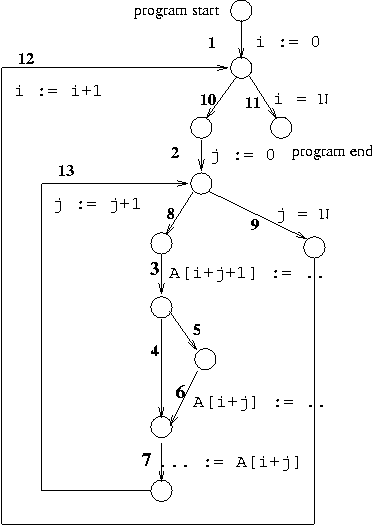
\includegraphics[scale=0.5]{images/cffada.png}
        \caption{Ablaufgraph}
        \vspace{+40pt}
    \end{flushright}

\end{wrapfigure}

\textit{Programmcode:}\\
    \begin{procedure}[H]
    \SetAlgoLined
    \For{$i=0$ \KwTo $N$}{
        \For{$j=0$ \KwTo $N$}{

            \textbf{3:} $A[i+j+1]$ = ... \\
            \eIf{$P$}
                {\textbf{6:} $A[i+j]$ = ...\\}{}
            \textbf{7:} ... = $A[i+j]$

        }
    }
    \end{procedure}

~\\[6cm]
\textbf{Kontext}\\
Read-Statement 7\\
Operationen: $\langle (i,j), 7 \rangle$ für $0 \leq i, j \leq N$\\
\\
\textbf{Annotierung}\\
Statement 3\\
Operationen: \(\langle (i^\prime,j^\prime), 3 \rangle\) für \( \underbrace{0 \leq i^\prime, j^\prime \leq N}_{Existenz} \land \underbrace{i^\prime + j^\prime + 1 = i + j}_{Konflikt}\)\\
Statement 6\\
Operationen: \dots\\

\textbf{Durchlauf}\\
\begin{enumerate}
    \item {Ordnung: \(i=i^\prime \land j=j^\prime\) \\
        \(src^{(0)} = {\perp}\)\\
        \begin{enumerate}
            \item Start: 7
            \item die 4 hoch: (Kante mit Label 4)\\
                  Keine neuen Quellen\\
                  \(scr_{4}^{(1)} = \lbrace \perp \rbrace\)
            \item die 6 hoch: (überprüfe Existenzun- und Konfliktgleichungen)\\
                  \(src_{6}^{(1)} = src^{(0)} \Box W(6) = \)
    \(\begin{cases}  \langle (i,j), 6 \rangle , & \mbox{ für } P^\prime(i,j) \\
                     \perp ,                    & \mbox{ sonst }
    \end{cases}  \)

            \item bei n1 Mischen:\\
                \(scr_{n1}^{(1)} =
    \begin{cases} \langle (i,j),6 \rangle, & \mbox{ für } p^\prime(i,j) \\
                  \perp,                   & \mbox{ sonst }
                \end{cases} \)

            \item die 3 hoch:\\
                  Keine neuen Quellen, da die aktuelle Ordnung $\lightning$ Konfliktgleichung. (Wäre P immer true, könnte man an n1 abbrechen.)
            \item die 13 hoch \(\Rightarrow\)

        \end{enumerate}
        }
    \item {Ordnung: \(i=i^\prime \land j^\prime < j\) \\
      \begin{enumerate}
         \item die Kanten 7, 4 bringen nichts neues.
         \item die 6 hoch: \\
           Keine neuen Quellen, da die aktuelle Ordnung $\lightning$ Konfliktgleichung.
         \item n1: nichts neues zu mischen \(\Rightarrow\) alles bleibt
         \item die 3 hoch: \\
           \(src^{(2)} = src^{(1)} \Box W(3) = \) \\ \( =
           \begin{cases} \langle ( i^\prime, j^\prime), 3) \rangle, & \mbox{ für } i^\prime + j^\prime + 1 = i + j \land \neg P^\prime(i,j) \land 0 \leq i^\prime \leq N \land 0 \leq j^\prime \leq N \\ & \mbox{ mit aktueller Ordnung}\\
             \langle (i,j),6 \rangle , & \mbox{ für } P^\prime(i,j) \\
             \perp, & \mbox{sonst}
           \end{cases}
\)
           \\ \(\stackrel{j^\prime+1=j}{=}
           \begin{cases}
             \langle ( i, j-1), 3 \rangle, & \mbox{ für }\neg P^\prime(i,j) \land j > 0 \land 0 \leq j-1 \leq N \\
             \langle (i,j),6 \rangle , & \mbox{ für } P (i,j) \\
             \perp , & \mbox{ sonst, d.\,h. } j = 0 \land \neg P(i,0)
           \end{cases}
           \)
         \item Kante 8: -
         \item Kante 2: -
         \item Kante 10: -
         \item Kante 12: -
      \end{enumerate}
      }

      \item {Ordnung: \(i^\prime < i, j^\prime\) beliebig
          \begin{enumerate}
            \item Kante 9,13,7,4: -
            \item Kante 6: \\
              wegen Optimierung: \(j= 0 \land \neg P^\prime (i,j)\) \\
              Ordnung: \(i^\prime < i \) \\
              Konflikt: \( i^\prime + j^\prime = i + 0 \) \\
              Existenz: \( P^\prime(i^\prime, j^\prime) \) \\
              neue Quellen: \( \langle ( i^\prime, i-i^\prime ), 6 \rangle \text{ für } j=0, i^\prime < i , P(i^\prime, i - i ^\prime) \land \neg P(T, i-T) \text{ für } i^\prime < T \leq i \) \\

\( src^{(3)}_{n1} =
\begin{cases}
  \langle (i,j), 6 \rangle, & \mbox{ für } P(i,j) \\
  \langle (i,j-1), 3 \rangle, & \mbox{ für } j \geq 1 \land \neg P (i,j) \\
  \langle (i^\prime, i-i^\prime),6 \rangle, & \mbox{ für } j=0 \land i^\prime < i \land P(i^\prime, i - i^\prime) \land \neg P(T,i-T) \\ & \mbox{ für } i^\prime < T \leq i \land i^\prime \geq 0 \land i \geq 1 \\
  \perp, & \mbox{ für } j=0 \land \neg P(i^\prime, i - i^\prime) \text{ für alle } 0 \leq i^\prime \leq i
\end{cases} \)

\item Kante 3:\\
  wegen Optimierung: \( i^\prime = i - 1, j=0 \stackrel{Konfl. Gl.}{\Rightarrow} j^\prime = 0\) \\
  neue Quelle: \( \langle (i-1,0), 3 \rangle \text{für} j=0 \land i \geq 1 \land \neg P(i,0) \land \neg P(i-1,1) \) \\
\( \Rightarrow src =
\begin{cases}
  \langle (i, j), 6 \rangle, & \mbox{für } P(i,j) \\
  \langle (i, j-1), 3 \rangle, & \mbox{für } j \geq 1 \land \neg P(i,j) \\
  \langle (i-1, 1), 6 \rangle, & \mbox{für } j=0 \land \neg P(i,j) \land P(i-1,1) \\
  \langle (i-1, 0), 3 \rangle, & \mbox{für } j=0 \land \neg P(i,j) \land \neg P(i-1,1) \land i \geq 1 \\
  \perp, & \mbox{für } i=j=0 \land \neg P(0,0)
\end{cases}
\)
\item Kanten 8, 2, 10, 1: -
           \end{enumerate}
           }

\end{enumerate}
Da die Quelle für \( (0,0) \) nicht gefunden wird, kann nicht vorab abgebrochen werden und der Algorithmus terminiert erst mit dem vollständigen Durchlauf.
    \begin{itemize}
        \item ...
        \item Single-Assignment-Konversion
    \end{itemize}
\subsubsection{Vereinfachte Abhängigkeitsanalyse}
    \begin{itemize}
        \item GCD (einfach und erweitert)
        \item Extreme-Value-Test
    \end{itemize}


\subsubsection{Normalisierung der Array-Indizes}

Einfache Abhängigkeitsanalyse macht keine symbolische Auswertung,
insbesondere setzt sie Skalarvariablen, die als Arrayindizes auftreten,
nicht ein, obwohl man deren Wert manchmal bestimmen kann. Beispielsweise
wäre im folgenden Programm jede Instanz der Array-Zuweisung von jeder
anderen ausgabeabhängig, weil der Arrayindex $x$ als unbekannt
angenommen wird:

% {\sf\begin{tabbing}
% \ins\=\ins\=\ins\=\ins\=\ins\=\kill
%   for $i := 1$ to $n$ do\\
%   \> $x := 2*i+4$;\\
%   \> $A[x] := ...$;\\
%   enddo
% \end{tabbing}}

\begin{procedure}
\SetAlgoLined
\For{$i:= 1$ \KwTo $n$}{
     $x := 2 \cdot i+4$;\\
     $A[x] := ...$;\\
}
\end{procedure}

\paragraph{Skalar-Vorwärts-Ersetzung}
\label{sec:sve}

Direktes Einsetzen der Definition des Skalars in den Arrayindex liefert
das linke Programm. ACHTUNG: Gültigkeitsbereiche beachten! Im rechten
Programm ist das Ersetzen des Arrayindexes $j$ durch seine Definition
$i+1$ \emph{verboten} (vgl. \cite{Zima90}, S.~178 f.):\\[1cm]
\begin{minipage}{.4\textwidth}
    \begin{algorithm}[H]
        \For{\( i:= 1 \) \KwTo \( n \)}{
               $x := 2 \cdot i+4$;\\
               $A[2 \cdot i+4] := ...$;\\
        }
    \end{algorithm}
\end{minipage}
\begin{minipage}{.4\textwidth}
    \begin{algorithm}[H]
    $j := i+1$;\\
    $i := 0$;\\
    $A[j] := ...$;\\
    \end{algorithm}
\end{minipage}

\paragraph{Beispiel}

\begin{procedure}[H]
\SetAlgoLined
\For{$i=..$ \KwTo $n$}{
	$x=2i+4$ \\
		 ...  = \(A[x]\)  \\
}
\end{procedure}
Abhängigkeit: $i \rightarrow i+1$ schon wegen $x$

$\leadsto$

\begin{procedure}[H]
\SetAlgoLined
\For{$i=1$ \KwTo $1000$}{
	 	   ... = \(A[2i+4]\)
}
\end{procedure}

$\Rightarrow$ keine Abhängigkeit
\newpage
\paragraph{Wrap-Around-Variablen-Ersetzung}
\label{sec:wave}

Ähnlich zu Fall \ref{sec:sve}; allerdings ist die Skalar-Definitioin
textuell nach dem Arrayzugriff.

Das Problem ist einfach mit \emph{loop rerolling} zu lösen, wenn die
Initialisierung ``zum Schleifenprogramm paßt''; im allgemeinen ist aber
\emph{loop peeling} nötig, um Unregelmäßigkeiten an den Schleifengrenzen
zu beseitigen. Den Hauptanwendungsbereich für diese Transformation
bilden zyklische Arrays (daher wrap-around; vgl. \cite{Zima90}, S.~183).

Beispiel: Wenn $c=2$ ist, dann ist das linke Programm  äquivalent zu dem
mittleren; ansonsten ist es nur äquivalent zu dem rechten Programm:\\

\begin{minipage}[c]{4cm}
\begin{algorithm}[H]
    \( x := c \);\\
    \For{\( i:= 0 \) \KwTo \( n \)}{
        \( A[x] := \dots \);\\
        \( x := 2 \cdot i + 4 \);
    }
\end{algorithm}
% {\sf\begin{tabbing}
% \ins\=\ins\=\ins\=\ins\=\ins\=\kill
%   $x := c$;\\
%   for $i := 0$ to $n$ do\\
%   \> $A[x] := ...$;\\
%   \> $x := 2*i+4$;\\
%   enddo\\
% \end{tabbing}}
\end{minipage}
\begin{minipage}[c]{4cm}
\begin{algorithm}[H]
    \For{\( i:= 0 \) \KwTo n}{
        \( x := 2 \cdot i + 4 - 2 \);\\
        \( A[x] := \dots \);
    }
    \( x := 2 \cdot n + 4 \);
\end{algorithm}
% {\sf\begin{tabbing}
% \ins\=\ins\=\ins\=\ins\=\ins\=\kill
%   for $i := 0$ to $n$ do\\
%   \> $x := 2*i+4-2$;\\
%   \> $A[x] := ...$;\\
%   enddo\\
%   $x := 2*n+4$;\\
% \end{tabbing}}
\end{minipage}
\begin{minipage}[c]{4cm}
    \begin{algorithm}[H]
        \( A[c] := \dots \);\\
        \For{\( i := 1 \) \KwTo \( n \)}{
            \( x := 2 \cdot i + 4 - 2 \);\\
            \( A[X] := \dots \);
        }
        \( x := 2 \cdot n + 4 \);
    \end{algorithm}
% {\sf\begin{tabbing}
% \ins\=\ins\=\ins\=\ins\=\ins\=\kill
%   $A[c] := ...$;\\
%   for $i := 1$ to $n$ do\\
%   \> $x := 2*i+4-2$;\\
%   \> $A[x] := ...$;\\
%   enddo\\
%   $x := 2*n+4$;
% \end{tabbing}}
\end{minipage}


\paragraph{Induktions-Variablen-Ersetzung}
\label{sec:ive}

Einfache Induktionsvariablen sind Variablen, denen nur durch (ggfs.
mehrere) Terme $v := v + c_0$ Werte zugewiesen werden; allgemeine
Induktionsvariablen sind Variablen, denen einmalig mit einem Term der
Form $v':= c_1*v + c_2$ ein Wert zugewiesen wird, wobei $v$ eine
einfache Induktionsvariable sein muß.  Sie können stets durch einen
affinen Ausdruck in den Schleifenindizes
ersetzt werden:\\

\begin{minipage}[c]{4cm}
    \begin{algorithm}[H]
        \( x:= 2 \);\\
        \For{\( i:=0 \) \KwTo \( n \)}{
            \( x := x+2 \);\\
            \( A[x] := \dots \);
        }
    \end{algorithm}
% {\sf\begin{tabbing}
% \ins\=\ins\=\ins\=\ins\=\ins\=\kill
%   $x := 2$;\\
%   for $i := 0$ to $n$ do\\
%   \> $x := x+2$;\\
%   \> $A[x] := ...$;\\
%   enddo
% \end{tabbing}}
\end{minipage}
%
\begin{minipage}[c]{4cm}
\centerline{ist äquivalent zu}
\end{minipage}
%
\begin{minipage}[c]{4cm}
    \begin{algorithm}[H]
        \For{\( i:= 0 \) \KwTo \( n \)}{
            \( x:= 2 \cdot i + 4 \);\\
            \( A[x] := \dots \);
        }
    \end{algorithm}
% {\sf\begin{tabbing}
% \ins\=\ins\=\ins\=\ins\=\ins\=\kill
%   for $i := 0$ to $n$ do\\
%   \> $x := 2*i+4$;\\
%   \> $A[x] := ...$;\\
%   enddo
% \end{tabbing}}
\end{minipage}

\bigskip
Anschließend an \ref{sec:wave} und \ref{sec:ive} kann man \ref{sec:sve}
anwenden, und schließlich kann man das entstandene Programm mit Hilfe von
\emph{Dead-Code-Eliminierung} noch vereinfachen.


\def\ins{\hspace{.5cm}}

\subsection{Eliminieren von Abhängigkeiten}

\subsubsection{Scalar Renaming}

Anti- und Output-Abhängigkeiten können u.U. durch einfaches Umbenennen
von Variablen eliminiert werden. Zentrale Technik: Ermitteln der
``erreichenden Definitionen''.

\paragraph{Beispiel}



\[
\begin{array}{ccc}
\begin{aligned}
A &= ... \\
   &= A \\
   &= A \\
A &= ... \\
   &= A
\end{aligned}
&
\leadsto
&
\begin{aligned}
A &= ... \\
   &= A \\
   &= A \\
A^\prime &= ... \\
   &= A^\prime
\end{aligned}
\end{array}
\]



\subsubsection{Scalar Expansion}

Schleifengetragene Anti- und Output-Abhängigkeiten von nicht voll
indizierten Variablen können durch volle Indizierung der Variablen
eliminiert werden (vgl. Single-Assignment-Konversion).

%\mg{Bsp: zweifach verschachtelt, einmal unwirksam, einmal gut, die volle
%  Indizierung}

\paragraph{Beispiel}
\begin{minipage}{.4\textwidth}
\begin{algorithm}[H]
\SetAlgoLined
\For{$i=1$ \KwTo $1000$}{
        A = ... \\
		   = A \\
	 	   = A
}
\end{algorithm}
\end{minipage}
\begin{minipage}{.5\textwidth}
\qquad $\leadsto$ \qquad
\begin{algorithm}[H]
\SetAlgoLined
\For{$i=1$ \KwTo $1000$}{
        \(A[i]\) = ... \\
		   = \(A[i]\)  \\
	 	   = \(A[i]\)
}
\end{algorithm}
\end{minipage}
\subsubsection{Variable Copying}

Antiabhängigkeiten kann man u.U. durch eine vorab erstellte Hilfskopie
des Arrays einfach eliminieren.

\paragraph{Beispiel}
\begin{minipage}{.4\textwidth}
\begin{procedure}[H]
\SetAlgoLined
\For{$i=0$ \KwTo $n$}{
        $A[i]$ = ... \\
		   = $A[i] + A[i+1]$ \\
}
\end{procedure}
\end{minipage}
\qquad $\leadsto$ \qquad
\begin{minipage}{.5\textwidth}
\begin{procedure}[H]
\SetAlgoLined
\For{$i=0$ \KwTo $n$}{
        $A^\prime[i]$ = $A[i+1]$ \\
}
\end{procedure}

\begin{procedure}[H]
\SetAlgoLined
\For{$i=0$ \KwTo $n$}{
                $A[i]$ = ... \\
		   = $A[i] + A^\prime[i]$ \\
}
\end{procedure}
\end{minipage}

\subsubsection{Index Set Splitting}

Wenn die Abhängigkeit in unterschiedlichen Teilen des Indexraumes
verschieden ist, dann kann man u.U. die Schleifen so aufteilen, daß
schleifengetragene Abhängigkeiten eliminiert werden.

\subsubsection{Single-Assignment-Konversion}

\begin{enumerate}
	\item Feautriers Abhängigkeitanalyse laufen lassen  \( \leadsto \) \glqq Datenfluss\grqq
	\item Jedes \glqq write\grqq\ wird zu einem neuen \glqq write\grqq\ in ein neues, voll indiziertes Array.
	\item Jedes \glqq read\grqq\ wird ersetzt durch sein \dots %fehlt
	gemäß Datenfluss
\end{enumerate}

\subsubsection{Weitere Möglichkeiten}

Node splitting (komplexe Statements aufbrechen), loop peeling,
unrolling, rerolling (Unregelmäßigkeiten in den Schleifen eliminieren
und vorgegebene Statement-Reihenfolge ermöglichen) und idom recognition
(Mustererkennung zum Einsatz von Reduktionen).


\def\ins{\hspace{.5cm}}



\subsection{Ausgewählte Parallelisierungstechniken}

%Abschließend soll auf die einfachen Parallelisierungstechniken
%eingegengen werden. Die verallgemeinerten Verfahren werden im nächsten
%Semester noch einmal ausführlicher behandelt.

\subsubsection{Iteration Graph Partitioning}
\label{sec:igp}

Idee: \textit{Parallel kann ausgeführt werden, was nicht voneinander
abhängig ist}.

Die schwachen Zusammenhangskomponenten des
Iterations-Abhängigkeitsgraphen werden zueinander parallel und in sich
sequentiell ausgeführt.

Bei verschachtelten Schleifen berechnet man dazu für jede
Schleifendimension den größten gemeinsamen Teiler \textit{gcd} der
Abhängigkeitsvektoren. Grund: der Abhängigkeitsgraph zerfällt in gcd
viele unabhängige Teile (die Iterationen $i$, die durch $i$ modulo gcd
in unterschiedliche Klassen fallen, können nie voneinander abhängig
sein).

Anschließend kann man mechanisch jede Schleife durch ein Paar von
Schleifen ersetzen: eine parallele Schleife zählt die möglichen Werte
für ``Index modulo gcd'' auf und eine sequentielle die jeweils
auftretenden Resultate der ganzzahligen Division ``Index / gcd'' (\cite{Ban94},
124ff).

{\sffamily for $i:=x$ to $y$ do $R(i)$ enddo} wird, wenn der größte
gemeinsame Teiler der Abhängigkeitsvektoren der Dimension $i$ gleich
$g$ ist, zu

% {\sf\begin{tabbing}
% \ins\=\ins\=\ins\=\ins\=\ins\=\kill
%   forall $m := 0$ to $g-1$ do\\
%   \> for $d := \lceil{x-m\over g}\rceil$ to $\lfloor{y-m\over g}\rfloor$ do\\
%   \>\> $R(m+g*d)$\\
%   \> enddo\\
%   enddo
% \end{tabbing}}

\begin{algorithm}[H]
    \ForAll{\( m:=0 \) \KwTo \( g-1 \)}{
        \For{\( d:= \lceil{x-m\over g}\rceil \) \KwTo \( \lfloor{y-m\over g}\rfloor \)}{
            \( R(m+g \cdot d) \)
        }
    }
\end{algorithm}


\bigskip

Im folgenden nehmen wir der Einfachheit halber an, daß der zu
parallelisierende Schleifensatz perfekt verschachtelt ist.

\subsubsection{Schleifenpermutation}

Ideen: \textit{Eine Schleife kann parallel ausgeführt werden, wenn sie keine
Abhängigkeiten trägt}, und: \textit{Abhängigkeitsvektoren dürfen nie
negativ sein}.

Damit kann man zwei Schleifen genau dann vertauschen, wenn durch die
entsprechende Permutation im Richtungsvektor kein lexikographisch
negativer Richtungsvektor entsteht.

Wenn alle Abhängigkeiten (ggf. nach Permutation) durch eine Anzahl von
äußeren Schleifen getragen wird, dann kann man die inneren alle parallel
ausführen.

\subsubsection{Unimodulare Transformationen}

Idee: \textit{Durch Mischen (Scheren, ``skewing'') von einer (inneren)
Schleife in
eine andere (äußere) kann man die tragende Schleife einer Abhängigkeit
verändern}.

Im folgenden sei $m$ die Dimensionalität des Schleifensatzes. Um
konsistent mit dem Space-Time-Mapping-Ansatz zu sein
(Kapitel~\ref{sec:polymod}), multiplizieren wir Vektoren nun wieder von
rechts an die Transformationsmatrix (im Gegensatz zu \cite{Ban93, Ban94}
und dem Beschluß in Kapitel~\ref{sec:math:i}). Damit werden auch die
Abhängigkeitsvektoren zu Spaltenvektoren (im Gegensatz zur
vorangegangenen Abhängigkeits-Vorlesung).  Die \emph{Distanzmatrix}
(=\emph{Abhängigkeitsmatrix}) $\cal D$ ist dann eine
$m\!\times\!r$-Matrix, die spaltenweise aus den Distanzvektoren
(=Abhängigkeitsvektoren) $d_1,\cdots,d_r$ aufgebaut ist.

\subsubsection{Parallelisierung innerer Schleifen}

Im Fall von uniformen Abhängigkeiten kann man jedes Schleifenprogramm so
transformieren, daß alle Schleifen außer der äußersten Schleife parallel
sind. Die dazu nötige Transformationsmatrix wird so konstruiert, daß
alle Abhängigkeiten von der äußersten Schleife getragen werden.

Etwas präziser: es wird ein Vektor $u$ (erste Zeile der
Transformationsmatrix) gesucht, so daß
\begin{enumerate}
\item $gcd(u_1,\cdots,u_m) = 1$\\[-7mm]
\item $u_1*{\cal D}_{1k} + \cdots + {\cal D}_{mk}*u_m \geq 1$ für alle
  Abhängigkeitsvektoren $1\!\leq\!k\!\leq\!r$\\[-7mm]
\item $\max_{I\in \textrm{\small Indexraum}}(u*I) - \min_{I\in
    \textrm{\small Indexraum}}(u*I) + 1$ minimal
\end{enumerate}

Eine greedy-Heuristik, die sog. Hyperebenenmethode von Lamport,
berücksichtigt nur das erste und zweite Kriterium exakt und nähert das
dritte an.

\smallskip

Die gesamte Matrix wird dann konstruiert, indem man sie unimodular
ergänzt: trage den Vektor $u$ als erste Zeile in eine
$m\!\times\!m$-Matrix ein, streiche dann eine Spalte mit Eintrag eins in
der ersten Zeile (existiert bei Lamport's Verfahren) und die erste Zeile
selbst, und fülle den Rest mit der Einheitsmatrix der Dimension
$m\!-\!1$ auf. Zusammen mit den gestrichenen Einträgen ergibt sich dann
eine unimodulare Matrix (Determinante ist $\pm 1$).


\subsubsection{Parallelisierung äußerer Schleifen}
\label{sec:pas}

Wenn $\rho$ der Zeilenrang der Abhängigkeitsmatrix ist, dann kann man
nur $m\!-\!\rho$ viele äußere Schleifen in parallele Schleifen umwandeln.
Grund: da äußere Parallelschleifen keine Abhängigkeit tragen können,
dürfen alle transformierten Abhängigkeitsvektoren in den ersten Zeilen
nur Null-Einträge haben, d.h., $T*\cal D$ muß mit $m\!-\!\rho$
Nullzeilen beginnen. Da der Rang von $\cal D$ wegen der Unimodularität
von $T$ gleich dem Rang von $T*\cal D$ ist, muß $\cal D$ schon $m\!-\!\rho$
linear abhängige Zeilen besitzen.

Es ist dann allerdings möglich, alle Abhängigkeiten von der
$m\!-\!\rho\!+\!1$-ten Schleife tragen zu lassen, so daß wieder nur eine
einzige sequentielle Schleife im Zielprogramm nötig ist.

\subsubsection{Asynchronität}

Die soeben gemachte Feststellung scheint im Widerspruch zu der Aussage
zu stehen, daß man durch Wahl der Zielschleifenreihenfolge im
Space-Time-Mapping-Ansatz synchrone oder asynchrone (also jederzeit auch
$m\!-\!1$ äußere Parallelschleifen!) erreichen kann. Auflösung: beim
Space-Time-Mapping-Ansatz ist Kommunikation und/oder Synchronisation von
asynchron parallel arbeitenden Prozessoren erlaubt (``DOACROSS''), bei allen
anderen vorgestellten Methoden arbeiten parallele Prozessoren stets
unabhängig voneinander (``DOALL'').
%---die einzig mögliche Synchronisation die durch eine
% gemeinsam umgebende sequentielle Schleife (im Fall~\ref{sec:pas} nicht
% bedingt die äußerste).


\subsubsection{Loop Distribution}

Idee: \textit{Man gibt bei Bedarf jedem Statement seine eigenen
  Schleifen}.

Loop Distribution arbeitet als einziges der hier vorgestellten Verfahren
mit dem Statement-Abhängigkeitsgraphen. Im Gegensatz zu den unimodularen
Transformationen (aber ähnlich dem Iteration Graph Partitioning)
beinhaltet die Methode bereits die Code-Generierung. Diese Methode
arbeitet sehr effizient und liefert gute Ergebnisse.

Vorgehen (rekursiv über die Schleifendimensionen):\\[-3ex]
\begin{enumerate}
\item Berechne den Statement-Abhängigkeitsgraphen.\\[-4ex]
\item Berechne die \emph{azyklische Kondensation}, d.h. die starken
  Zusammenhangskomponenten und die darauf geltende Halbordnung.\\[-4ex]
\item Für jede starke Zusammenhangskomponente baue eine neue Schleife:
  sequentiell, falls eine Abhängigkeit existiert, parallel sonst.\\[-4ex]
\item Diese Schleifen werden gemäß der Halbordnung auf den
  Zusammenhangskomponenten sequentiell komponiert.\\[-4ex]
\item Entferne alle bereits berücksichtigten (von den soeben
  eingeführten sequentiellen Schleifen getragenen) Abhängigkeiten und
  fahre mit dem Restgraphen (und damit der nächst-inneren Dimension) bei
  2. fort.
\end{enumerate}

\subsubsection{Polyedermodell}

Das Polyedermodell stellt eine Vereinigung aller Verfahren innerhalb
eines mathematischen Frameworks dar. Etwas genauer: das Polyedermodell
ist eine Erweiterung des ursprünglichen Polytopmodells (des
Space-Time-Mapping-Ansatzes), allerdings mit stark erweiterter
Anwendbarkeit, z.B.  nicht-perfekte Verschachtelung, separate
Transformationen je Statement, die stückweise linear sein können,
allgemeine {\sffamily for}- und {\sffamily while}-Schleifen, {\sffamily if}-Anweisungen,
affine Abhängigkeiten, Ab\-schät\-zung der Abhängigkeiten bei nicht-affinen
Array-Indizes (s.~Kapitel~\ref{sec:polymod}). Der wesentliche Nachteil,
den man sich durch diese Flexibilität erkauft, ist eine aufwendige
Zielcodegenerierung (aufwendig sowohl zur Übersetzungs-, als auch zur
Laufzeit).
